\section{Method}

\subsection{Generalized Critic}



\ref{fig:model}

\subsection{Variations}

\subsubsection{Estimation methods for the value and advantage functions}

%method
%gamma and lambda

\subsubsection{Random initialization and bootstrap at training}

\subsubsection{Hyperparameters and optimizations}

\label{sec:meth}
\begin{algorithm}[H]
\DontPrintSemicolon
  
  \KwInput{Initial actor network parameters $\theta_0$, initial critic parameter list $\phi^0_0, \dots, \phi^n_0$}
  %\KwOutput{Your output}
  %\KwData{Testing set $x$}

  \For{$i \leftarrow 1$ \KwTo total number of updates}{     
\While{buffer is not full}{     
  \tcc{collect set of trajectories $\mathcal{D}_k$}
         Run $\pi_{\theta_{old}}$ to generate an action
         
         Store the current state, action, and reward in buffer
         
         \If{episode ends}
         	{break}
   }
   
\If{episode was interrupted}{
	bootstrap remaining values
   }

  \For{$i \leftarrow 1$ \KwTo number of critics}{
   Estimate the advantage functions $\hat{A_i}$ using any (or several) estimation methods}

   Compute the PPO-CLIP policy loss as: %formula
   
   Update the policy network

  \For{$i \leftarrow 1$ \KwTo number of critics}
    {
    	Update the value network $V_{\phi^1}$
    } 
}    
\caption{PPO-CLIP with Generalized Critic Policy Optimization}

\end{algorithm}

\begin{figure}[!htb]
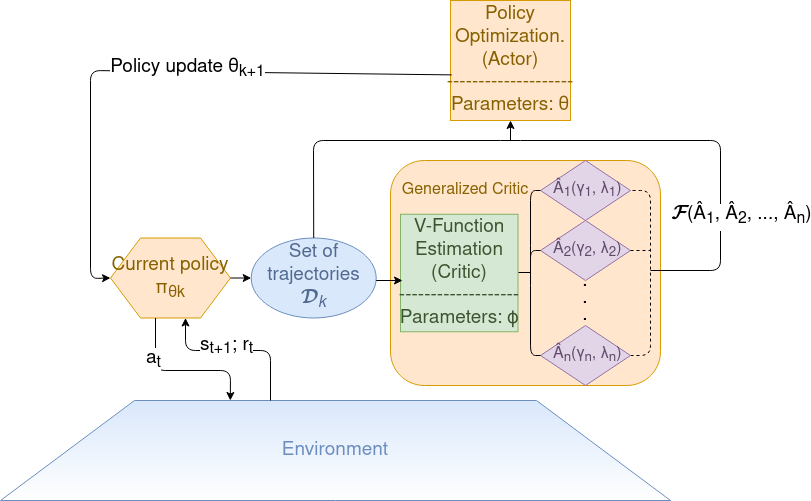
\includegraphics[width=\linewidth]{images/model}
\caption{Policy update scenario with a generalized critic.}
\label{fig:model}
\end{figure}
